\section {Best Ever Alarm System Toolkit - BEAST}

\subsection {Introdução} \label{beast-intro}

Em um ambiente composto por centenas de milhares de variáveis EPICS, como o que
será implementado no \textit{Sirius}, a necessidade de um sistema capaz de
monitorar quais variáveis encontram-se em estados errôneos torna-se
imprescindível. Sendo assim, o monitor de alarmes \textit{BEAST}, do inglês
\textit{Best Ever Alarm System Toolkit} e desenvolvido pelo laboratório
americano \textit{Oak Ridge National Laboratory}, representa uma solução capaz
de gerenciar e controlar os alarmes gerados pelos servidores EPICS disponíveis
na rede. Tal sistema é implementado em \textit{Java} e é baseado no ambiente
gráfico de desenvolvimento \textit{Eclipse}. A arquitetura do sistema
está represetada na figura \ref{fig:best_arquitetura}, logo abaixo.

\FloatBarrier

\begin{figure}[h]

\centering
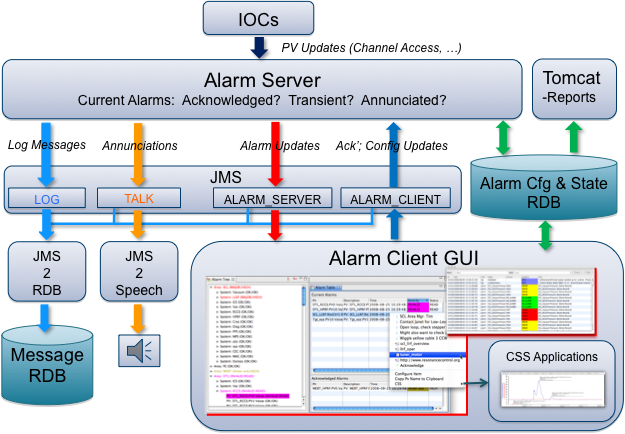
\includegraphics[scale=0.55]{image/beast-arquitetura}
\caption {Implementação do sistema de monitoramento de alarmes
\textit{BEAST}.}
\label{fig:best_arquitetura}
\end{figure}

\FloatBarrier

É possível distinguir diversos componentes na figura acima:

\begin{enumerate}[i.]
  
  \item \textit{Alarm server}: o servidor é responsável por tarefas fundamentais
  no monitoramento de alarmes. Cabe a ele a leitura da configuração dos alarmes
  armazenada no banco de dados \textit{Alarm Cfg \& State RDB}, conectar-se às
  respectivas variávies, monitorar suas mudanças de estado e gerar alarmes
  quando necessário e desativá-los logo que um operador toma conhecimento
  do problema. Esse módulo permite que um número variável de clientes se conecte
  a ele. Uma variável pode adotar duas configurações distintas, sendo elas
  \textit{latch} e \textit{annunciate}. Para a primeira, o servidor mantém o
  alarme de maior gravidade, mesmo que o estado da variável não seja
  atualmente errôneo, até que ele seja reconhecido manualmente pelo operador.
  A fim de impedir um grande volume de alarmes gerados, é possível habilitar
  as opções \textit{delay}, que aciona o alarme somente se o estado errôneo da
  variável se mantiver durante o intervalo de tempo especificado, e
  \textit{count}, que aciona o alarme se tal estado for detectado mais vezes
  que o valor especificado. A segunda configuração ativa o alarme somente
  quando a \textit{PV} apresentar valor inválido, sendo que ele é desativado
  logo que tal variável voltar à sua faixa de operação esperada.
  
  \item \textit{Alarm Cfg \& State RDB}: banco de dados relacional, como um
  servidor \textit{MySQL} por exemplo, onde serão armazenadas as configurações
  de alarme e o atual estado de todos os alarmes.
  
  \item \textit{Java Message Service - JMS}: utilizado para a comunicação entre
  diferentes módulos. No projeto, foi empregada a implementação realizada pelo
  \textit{Apache Software Foundation} chamada de  \textit{Apache ActiveMQ}. O
  sistema utiliza 4 \textit{topics} distintos, sendo eles:
  
  \begin{itemize} \renewcommand\labelitemi{--}
    \item \textit{ALARM\_SERVER}: utilizado pelo servidor para publicar
    atualizações nos estados dos alarmes de acordo com a configuração de cada
    variável.
    
    \item \textit{ALARM\_CLIENT}: permite que clientes notifiquem atualizações
    de configuração e reconhecimento de alarmes.
    
    \item \textit{TALK}: dedicado para anunciar mensagens.
    
  \end{itemize}
  
  \item \textit{Alarm Client GUI}: \label{client-gui} baseado na interface
  gráfica do \textit{Eclipse}, oferece três opções de monitoramento:
  
  \begin{itemize} \renewcommand\labelitemi{--}
    \item \textit{Alarm table}: mostra os alarmes em duas tabelas distintas
    contendo aqueles reconhecidos (\textit{acknowledged alarms}) e aqueles que
    ainda estão acionados (\textit{active alarms}).
    
    \item \textit{Alarm tree}: essa opção de visualização oferece
    uma visão hierarquica dos alarmes, sendo organizada, do nível mais alto para
    o menor, em áreas, sistemas, subsistemas e variáveis. Oferece opções para
    configurar, remover ou adicionar variáveis no nível desejado. O estado do
    alarme de cada item é mostrado por uma cor e por uma anotação, sendo
    composta por três sentenças entre parênteses, que representam
    respectivamente a gravidade atual (\textit{current severity}), a
    maior gravidade detectada anteriormente (\textit{alarm severity}) e o estado
    atual do alarme (\textit{alarm status}). É sincronizada diretamente ao banco
    \textit{Alarm Cfg \& State RDB}, o que implica que uma mudança realizada é
    rapidamente detectada pelo servidor e pelos demais clientes.
    
    \item \textit{Alarm area panel}: indicação gráfica do estado do sistema.
    
  \end{itemize}
  
  É possível, a partir de qualquer uma das \textit{views} presentadas acima,
  acessar outros recursos, como, por exemplo, gráficos e valores atuais das
  variáveis desejadas. Para isso, basta apertar com o botão direito acima da
  \textit{PV} e apertar em \textit{Process variables}.
  
  \vspace{12pt}
  
  A implementação fornece, ainda, suporte para autenticação de usuários via
  \textit{LDAP} ou \textit{JAAS}. Caso seja a escolha, somente usuários
  autorizados podem alterar as configurações de alarmes ou reconhecê-los.
  
  \item \textit{Web reports}: é fornecido também um conteúdo \textit{Web} capaz
  de gerar relatórios, calcular estatísticas (como, por exemplo, totais
  diários, variáveis que mais disparam alarmes, intervalos de tempo que os
  alarmes permanecem mais ativos em média \textit{etc.}) e monitorar os alarmes.
  Assim como os módulos do \textit{EPICS Archiver Appliance}, as páginas devem estar hospedadas em um
  servidor \textit{Tomcat}.
  
\end{enumerate}

\subsection{Instalação}

\textit{BEAST} necessita de uma base de dados relacional, de uma implementação
\textit{JMS} e de um ambiente gráfico baseado no \textit{Eclipse}. Utilizaremos,
respectivamente, o \textit{MySQL}, \textit{Apache ActiveMQ} e a versão
\textit{Eclipse Luna for RCP and Plugin Development}. Uma sugestão de instalação
é apresentada abaixo.

\begin{enumerate}[i.]
  \item  É necessário inicialmente fazer o \textit{download} do
  código fonte do \textit{CS Studio} para obter o produto relacionado ao \textit{Alarm server}.
  Para isso, acesse o repositório do projeto no \textit{GitHub} e extraia os
  arquivos em um diretório. Usaremos aqui o mesmo caminho especificado por
  \texttt{\$INSTALL\_DIR}, utilizado também na seção \ref{sec:archiver}.
  
  \begin{lstlisting}[language=bash, style=nonumbers]
$ cd $INSTALL_DIR/
$ wget https://github.com/ControlSystemStudio/cs-studio/archive/master.zip
$ unzip cs-studio-master.zip
$ rm cs-studio-master.zip
$ cd cs-studio-master/
\end{lstlisting}
   
   Na pasta \texttt{cs-studio-master/}, estão contidos todos os arquivos com os
   códigos-fonte do \textit{CS Studio}, porém só utilizaremos o diretório \texttt{applications/},
   que é o onde está a implementação do \textit{Alarm server}.
   
   \item \label{mysql-alarm} Antes de executar o servidor, é necessário primeiro
   configurar o banco de dados com as tabelas utilizadas por ele. Para isso, diversos
   \textit{scripts} de instalação são disponibilizados pelo desenvolvedor em 
   \texttt{applications/alarm/alarm-plugins/org.csstudio.alarm.beast/dbd}. Vamos
   usar parte do conteúdo contido em \texttt{ALARM\_MYSQL.sql}, uma vez que
   este arquivo adiciona algumas entradas nas tabelas, a fim de testar a
   aplicação. Abra este arquivo e comente as linhas a partir de \texttt{INSERT
   INTO ALARM.ALARM\_TREE VALUES (3, 2, 'System', now());}. As linhas acima
   desta sentença criam a hierarquia, que também nos será útil. Execute, então,
   os seguintes comandos:
   
\begin{lstlisting}[language=bash, style=nonumbers]
$ mysql -u root -p
>> CREATE DATABASE ALARM;
>> GRANT ALL ON ALARM.* TO 'lnls_alarm_user'@localhost IDENTIFIED BY 'alarm_password';
>> exit

$ mysql -u lnls_alarm_user -p
>> source applications/alarm/alarm-plugins/org.csstudio.alarm.beast/dbd/ALARM_MYSQL.sql;
\end{lstlisting}

Verifique que as tabelas foram criadas corretamente com:

\begin{lstlisting}[language=bash, style=nonumbers]
>> SHOW TABLES;
\end{lstlisting}
   
\item A próxima etapa é configurar o servidor de mensagens \textit{JMS}. Será
necessário fazer o \textit{download} do pacote \textit{Apache ActiveMQ}.

\begin{lstlisting}[language=bash, style=nonumbers]
$ cd $INSTALL_DIR/
$ wget http://www.apache.org/dyn/closer.cgi?path=/activemq/5.13.0/apache-activemq-5.13.0-bin.tar.gz
$ tar -xvzf apache-activemq-5.13.0-bin.tar.gz
$ rm apache-activemq-5.13.0-bin.tar.gz
$ cd apache-activemq-5.13.0/
\end{lstlisting}

O diretório \texttt{conf/} contem um arquivo, \texttt{activemq.xml}, com as
configurações do servidor. É possível, por exemplo, modificar a porta, que por
padrão é 61616, ou adicionar autenticação via \textit{jaas}. Para tal, adicione
as seguintes linhas neste arquivo.

\begin{lstlisting}[language=bash, style=nonumbers]
<plugins>
  <jaasAuthenticationPlugin configuration="PropertiesLogin" />
</plugins>
\end{lstlisting}

Neste caso, \textit{PropertiesLogin} é o nome da configuração contido no arquivo
\texttt{login.config}, que especifica os \textit{plugins} necessários e os
arquivos onde estarão armazenados os usuários, suas senhas (\texttt{users.properties}) e grupos
(\texttt{groups.properties}). Por fim, inicie o servidor com 

\begin{lstlisting}[language=bash, style=nonumbers]
$ cd $INSTALL_DIR/apache-activemq-5.13.0/bin/linux-x86-64/
$ ./activemq start
\end{lstlisting}

\item Tendo instalado os componentes responsáveis pela comunicação entre módulos
e base de dados de configurações, podemos iniciar o servidor. Para isso, vamos
utilizar a distribuição \textit{Luna} do \textit{Eclipse for RCP and RAP
Developers}, por apresentar melhor compatibilidade com os pacotes gráficos do
\textit{CS Studio}. Extraia e inicie a aplicação.

\begin{lstlisting}[language=bash, style=nonumbers]
$ cd $INSTALL_DIR/
$ wget http://www.eclipse.org/downloads/download.php?file=/technology/epp/downloads/release/luna/SR2/eclipse-rcp-luna-SR2-linux-gtk-x86_64.tar.gz
$ tar -xvzf eclipse-rcp-luna-SR2-linux-gtk-x86_64.tar.gz
$ rm eclipse-rcp-luna-SR2-linux-gtk-x86_64.tar.gz
$ cd eclipse/
$ ./eclipse
\end{lstlisting}

Importe o projeto que contem o servidor de alarmes. Para tal, entre em
\texttt{File > Import \ldots > General > Existing Projects into Workspace} e
escolha o diretório \texttt{\$INSTALL\_DIR/ applications/alarm/}. Dentro deste
projeto, abra o arquivo \texttt{AlamServer.product} contido em
\texttt{alarm-plugins > org.csstudio.alarm.beast.server}. Espera-se que uma tela
parecida com a figura \ref{img:product-view} seja aberta.

\FloatBarrier

\begin{figure}[h]

\centering
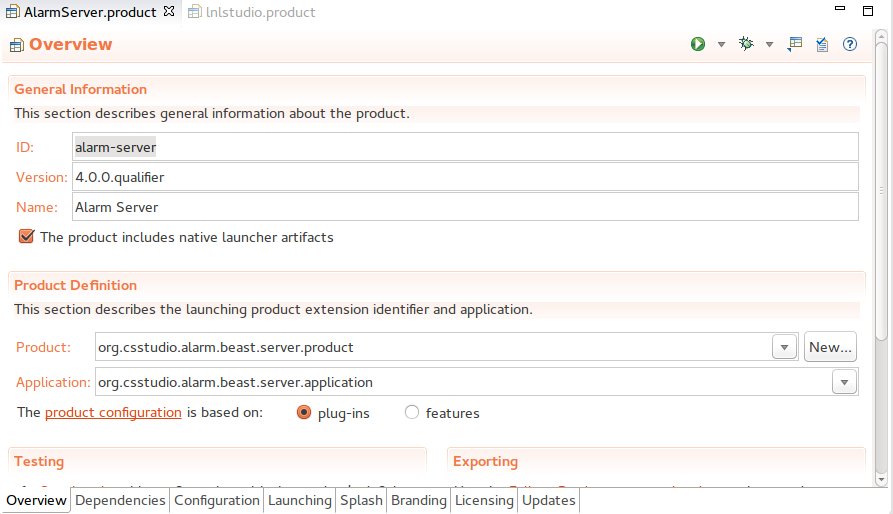
\includegraphics[scale=0.40]{image/product-view}
\caption {Configurações do produto \texttt{AlarmServer.product}.}
\label{img:product-view} 
\end{figure}

\FloatBarrier

Ainda não é possível executá-la, visto que este produto requer algumas
depedências. Para incluí-las à instalação do \textit{Eclipse}, acesse
\texttt{Help > Install New Software\ldots > Add\ldots} e adicione a \textit{url}
\textit{http://download.controlsystemstudio.org/updates/4.1}. Não é necessário
realizar o \textit{download} de todos os pacotes, somente os espeficados na
tabela \ref{tab:plugins} abaixo.

\FloatBarrier
\begin{longtable}[h] {| p{0.3\linewidth} | p{0.3\linewidth} | p{0.3\linewidth}   |}
\caption{\label{tab:plugins} \textit{Plugins} necessários para o
\textit{AlarmServer}.}\\
\hline \multicolumn{3}{| c |}{\textbf{CS-Studio Applications}} \\ \hline
\hline Alarm Handler Tools & Alarm Handler UI & Appliance Archiver Reader (x2) \\ \hline
Application Utilities & Archive Reader RDB Feature & Archive Tools Feature \\ \hline
CS-Studio Epics v3 Support & CS-Studio RAP Utilities & Data Browser \\ \hline
Data Browser OPI Widget & ea4 Archiver Reader & \\ \hline \hline
\multicolumn{3}{| c|}{\textbf{CS-Studio Core}} \\ \hline \hline
Core Auth Feature & Core Base Feature & Core Platform plugins   \\ \hline
Core Platform RAP Plugins & Core UI Feature & Core Utility Feature \\ \hline
CS-Studio Command-line Execution Services Support & CS-Studio Common Data
Layer (pvmanager) & CS-Studio DAL \\ \hline
CS-Studio Epics v4 Support & CS-Studio Extras Support & PVManager
Autocomplete Featue \\ \hline \hline
\multicolumn{3}{| c|}{\textbf{Maven osgi-bundles}}  \\ \hline \hline
antlr & EPICS Plug-in & Graphene \\ \hline
JSON support for file datasource & JSR 353 API & JSR 353 Default Provider \\ \hline
org.antlr.runtile & org.epics.graphne & org.epics.util \\\hline
org.epics.vtype & org.epics.vtype-json &  org.python.jython \\\hline
pvAccess - Java & pvData - Java &  PVManager Core \\\hline
PVManager EPICS Channel Access Support  & PVManager EPICS PVAccess Support  & 
PVManager Execute Support \\\hline
PVManager File Support  & PVManager Local PV Support  & 
PVManager Simulated PV Support \\\hline
PVManager System Support  & PVManager VType Support  & \\\hline
\end{longtable}
\FloatBarrier

O produto necessita também do \textit{plug-in} \texttt{com.ibm.icu.base} contido
no repositório \textit{Orbit}, acessado através do \textit{link} abaixo.
Selecione somente o pacote \textit{Internacional Components for Unicode for
Java (ICU4J)} e instale-o.

\begin{center}
\textit{http://download.eclipse.org/tools/orbit/downloads/drops/R20150124073747/repository/}
\end{center}

O servidor já pode ser executado, porém ele utilizará uma configuração padrão
para conectar-se ao \textit{MySQL} e ao \textit{JMS}. A fim de modificar tal
configuração, editamos o arquivo \textit{plugin\_ customization.xml}, presente
no mesmo diretório. Esse arquivo deve refletir as instalações realizadas
anteriormente. 

\vspace{12pt}

Entre na aba \texttt{Launching} e adicione o argumento
\texttt{-pluginCustomization} no campo \textit{Program Arguments}. Tal argumento
deve conter o caminho do arquivo \textit{plugin\_customization.xml}, conforme
figura abaixo.

\FloatBarrier

\begin{figure}[h]

\centering
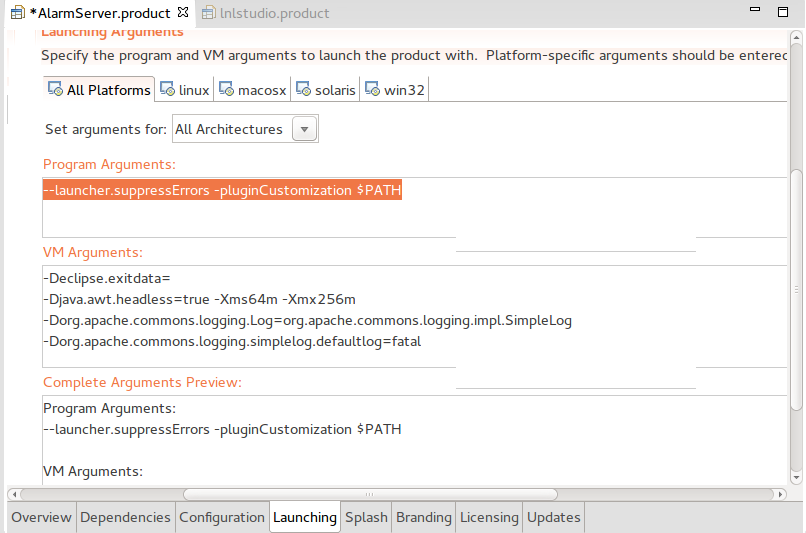
\includegraphics[scale=0.40]{image/launch-view}
\caption {\textit{Launching view} do produto \texttt{AlarmServer.product}.
Substituir \texttt{\$PATH\_TO\_FILE}} pelo caminho completo do arquivo
\textit{plugin\_customization.xml}.
\label{img:launch-view} 
\end{figure}

\FloatBarrier

Execute, enfim, o produto apertando no ícone verde no canto superior direito.
O servidor se encarregará da criação dos \textit{topics} na aplicação
\textit{JMS}. O resultado esperado está representado na figura
\ref{fig:server-on}. \textit{Annunciator} é o nome dado à raíz da hierarquia
criada no item \ref{mysql-alarm} e define, assim, quais tópicos serão
utilizados na comunicação.

\FloatBarrier

\begin{figure}[h]

\centering
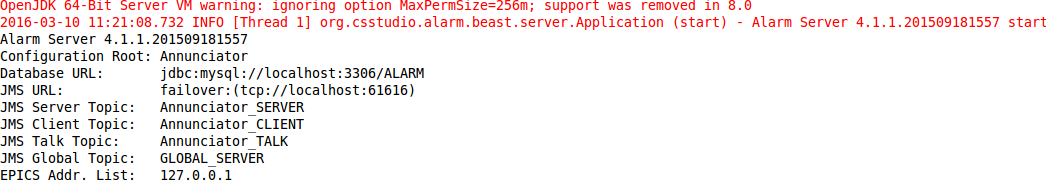
\includegraphics[scale=0.45]{image/alarmserver-on}
\caption {\textit{Launching view} do produto \texttt{AlarmServer.product}.
Substituir \texttt{\$PATH\_TO\_FILE}} pelo caminho completo do arquivo
\textit{plugin\_customization.xml}.
\label{fig:server-on} 
\end{figure}

\FloatBarrier

\end{enumerate}

\subsection{Uso da interface \textit{Eclipse} como \textit{Alarm Client GUI}}

Para configurar o \textit{Eclipse} como um cliente do servidor de alarmes, é
necessário configurá-lo para que ele acesse os servidores \textit{MySQL} e
\textit{JMS}. Isso é realizado através de \texttt{Window > Preferences > CSS
Applications > Alarm > Alarm System}. Modifique os campos\footnote{\textit{RDB}
significa \textit{Relational Database}, como o banco de dados \textit{MySQL}.}
\textit{url}, \textit{username} e \textit{password}, conforme configurado
anteriormente, e reinicie o \textit{Eclipse}. Se tudo foi configurado
corretamente, já é possível acessar os alarmes configurados através do
componentes comentados no item \ref{client-gui} da seção \ref{beast-intro}. Tais
componentes são acessados a partir de \texttt{Window > Show View > Other > CSS}.


\subsubsection {\textit{Debugging}} 

Alguns erros foram encontrados durante a instalação:

\begin{enumerate}[i.]
  \item \textit{A interface não salva corretamente as senhas do banco de dados e
  do JMS}: para resolver este problema basta redefir as senhas que o
  \textit{Eclipse} utiliza para criptografar as senhas salvas. Acesse
  \texttt{Window > Preferences > General > Security > Secure Storage} e redefina
  as senhas contidas na tabela \textit{Master password providers}.

  \item \textit{Não é possível adicionar, remover ou configurar variáveis a
  partir da Alarm Tree View}: conforme explicado na seção \textbf{Introdução}, o
  \textit{BEAST} oferece suporte à autenticação e autorização de usuários. Sendo
  assim, somente usuários cadastrados são permitidos de alterar ou reconhecer
  alarmes. Como a rede do \textit{Sirius} é prevista para ser isolada, tal
  serviço não será necessário. Portanto, podemos configurar o \textit{Eclipse}
  para dar permissão completa a qualquer \textit{user}. Para tal, devemos
  modificar o plugin \texttt{org.csstudio.security}, de extensão \textit{.jar}
  presente no diretório \textit {\$INSTALL\_DIR/eclipse/plugin}. Abra esse
  arquivo com o \textit{Archive Manager} (em sistemas \textit{linux}),
  modifique o campo \texttt{alarm\_config} para \texttt{.*} no arquivo
  \texttt{authorization.conf} e reinicie o \textit{Eclipse}. Deve ser possível
  alterar configurações de alarmes a partir de agora.
\end{enumerate}

\subsubsection {Obtendo um \textit{LNLStudio} a partir configuração do
\textit{Eclipse}}

É possível exportar a configuração atual do \textit{Eclipse} como um novo
produto, que chamaremos de \textit{LNLStudio}.
